 % Chapter Template

\chapter{Evaluation} % Main chapter title

\label{Chapter4} % Change X to a consecutive number; for referencing this chapter elsewhere, use \ref{ChapterX}

In order to evaluate this project we are going to compare the proposed architecture with the existing EPIC architecture in reliability and scalability as well as performance and real time delivery as proposed in the problem statement. We will also evaluate manteinability and future software development.

\section{Reliability}

To analyze reliability between systems we will analyze how well each system recovers if a components fails. We are interested to see how much time does it take to have the system recover if something failed. In addition we want to check what mechanisms do we have in both cases to check the health of each component. This would be useful to restart parts that have stopped working. 

\subsection{Current infrastructure}

Reliability on the existing EPIC infrastructure needs to be studied separately between EPIC Collect and EPIC Analyze. Collect is designed to be highly available. Using different techniques like cron jobs  that check the state and other. EPIC Collect is a really reliable system. It has been available 99\% of the time since 2012, making it really reliable for analysts to trust that their tweets are being collected. In the worst case scenario, EPIC Collect takes X seconds to recover. This is due the fact that the cron job that checks that EPIC Collect is running is scheduled every 5 seconds.

EPIC Analyze doesn’t have the same availability. The system has suffered multiples upgrades and depends on different pieces that can fail. Analyze depends on a separated Cassandra with Solr as well as a Redis cluster. If any of those two were to fail, the system would go down, being completely unusable. There’s no automatic recovery procedure. 

In conclusion, the current EPIC infrastructure depends of what secure layers developers have added to their programs, which makes it hard to develop and costly to keep it reliable. In addition, the deployment of the system is manual, which could involve human errors on deployment that could cause future instability of the system. This could be caused because components overlap each other RAM usage causing a full node of the cluster to go down.

\subsection{Proposed infrastructure}

In this case, reliability is a responsibility from the container orchestrated system. In our case, Kubernetes includes a controller manager on the master node. This component of the cluster keeps track of the status of each one of the containers running. The controller manager makes sure that a certain amount of replicas are up and running. If any container stops running at some point, the controller manager will make sure to schedule a new container and run it on an available node. This check is done on demand when there are new deployments requested or whenever a node notifies that a container is down.

 In addition to the controller manager, we also have the scheduler. This component makes sure that new container are scheduled in the best node possible. Kubernetes allows you to configure the amount of memory and cpu usage permitted by container, allowing the scheduler to find the best fit for each deployment request. 

Thanks to this deployment automation, node failures can be avoided easily as well as resources get a more optimized usage than if doing this process manually. Finally something else that Kubernetes allows to do natively is to rollout new versions of a service with no downtime. To do so the controller manager deploys the new version before removing the previous.  This is really useful for example in the Twitter tracker module, as this way all tweets get tracked even when the keywords change. In this case, the controller manager deploys a new version with the new keywords updated. Once it starts to run, it kills the previous version, which means that there’s always at least one version running and tracking all tweets. This ensures that we can get all tweets.

To test it, we left the system tracking for 11 days with no interaction from the user. As we can observe in Figure~\ref{fig:pods}, each instance has restarted many times. This could be caused when the  system reached peaks of load. With the limited amount of resources availables, Kubernetes has to kill some containers to avoid the whole system collapsing. Note that some instances say that have been existing for less than 2 days, this is due the fact that Kubernetes will restart the count if it needs to do a hard restart.



\begin{figure}
\centering
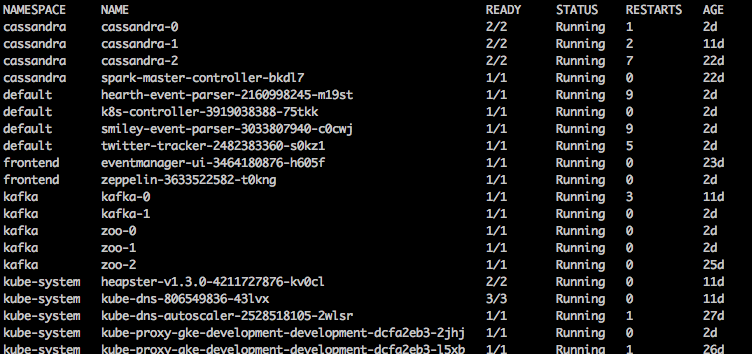
\includegraphics[width=\textwidth]{Figures/pods}
\decoRule
\caption[Status instances]{Status instances after 11 days}
\label{fig:pods}
\end{figure}

\section{Scalability}

We want a system that adapts to our needs, so we want a high scalability for it. We want to avoid wasting resources unnecessarily as well, so we want to be able to fit our available infrastructure. To analyze this we will see how easy is to scale each system and how scaling affects performance in either infrastructure.

\subsection{Current infrastructure}

The current infrastructure is not easy to scale. If we need to scale EPIC Collect, we would need to run manually a new instance, add cron jobs as well as add new Twitter credentials for it. This is one of the reason why EPIC Collect doesn’t do data normalization, if we added data normalization to the current EPIC Collect then on traffic spikes the system could be overloaded and would not be able to scale during high demand tweet incoming. 

Regarding storage, scalability is high thanks to Cassandra. Adding new nodes to the cluster it’s a pretty straight forward process. However regarding it will be difficult to add more Cassandra nodes than machines we have available, due to the fact that we will need to add more open ports to the outside of the machine. This is a small step back, as it’s not really complex. 

Regarding EPIC Analyze, the only thing we could scale, apart from storage, would be the frontend module. However that would mean adding a standalone load balancer in front of the service, which makes it a complex process if done manually and adds more complexity to maintain it. Also, we would need to add an external component to keep session information consistent across all the replicas, even though we could reuse the current Redis cluster to do so. The application would still need a refactor either way. 

In conclusion, it’s not really easy to scale the current infrastructure.

\subsection{Proposed infrastructure}

On the other side, the proposed architecture has a better and easy way to scale thanks to Kubernetes.

When deploying a service we can specify how many replicas we want to deploy. The controller manager will try to schedule as many replicas as it has been specified if there are enough resources. In addition, we tried to approach the design of the different components in a stateless way so that deploying new replicas would not require any additional change in the components. To achieve this, we moved the state to the infrastructure. The components are unaware of the state of the system, which makes it easy to add replicas. When added they do their task independently.

We could  also easily automate scalability  for each component depending on their CPU usage. If a certain container is in 90\% of their CPU usage, we can make that the system increments the number of replicas. This way the underlying resources can be administered in regards of the current needs of the system.

In terms of time to scale, it’s a matter to send the changes to Kubernetes. This can be done with a single command thanks to the command line tool kubectl or using the web interface for Kubernetes. Scaling is an integrated tool into container orchestrated systems, specially Kubernetes.

\section{Performance}

In order to analyze performance between both systems we need to take into account resources availables. All the analysis has been performed in the previously deployed 4 node cluster, each one with 4Gb or RAM and 1 virtual CPU. We will measure time to execute a word count script for a  certain number of collected tweets. We chose word count as it’s a highly a parallelizable program. 

Regarding performance we need to take into account different aspects. The current EPIC architecture performs really well when asking for some very specific queries. However, if we want more general queries or complex ones we would have to download the dataset to work with it with local tools, which makes analysis way slower. 

The goal for the architecture should be to give tools for analysts to develop their work without having to wonder how it was implemented. For this reason I focused on delivering a query flexible system that let’s query data in different ways. 

In order to analyze the performance in an overall way, we will take an example of dataset collected in the current infrastructure and one in a WordCount exercise. I selected WordCount as it’s a simple to describe data analysis and it has a high degree of parallelization. This way we can see how each system takes advantages of the distributed system.

In the new infrastructure we can use Spark running on top of Cassandra. This work should be optimized thanks to having a spark worker on each cassandra node, minimizing all network traffic by using data locality. 


\begin{lstlisting}[language=scala, caption={WordCount Spark script},float, floatplacement=H]
val table = sc.cassandraTable("twitter_analytics", "tweet")
val words = table.select("t_text").flatMap(l => l.getString("t_text").split(" "))
      .map(word => (word.toLowerCase,1)).reduceByKey(_ + _).map(_.swap).sortByKey(false,1)
\end{lstlisting}



To check how the query is performed we will look into the debug string from Spark. This is string is used to check how Spark will execute a query into its cluster. Each indentation is a map stage, and each + is a shuffle phase. As we can see in Listing~\ref{lst:rddebug}, Spark is not doing any shuffles until the reduce stage, meaning that it’s optimizing the query to take advantage of data locality by executing maps on the same node that the data is loaded to.



\begin{lstlisting}[language=scala, caption={Debug string rdd}, float, floatplacement=H, label={lst:rddebug}]
(1) ShuffledRDD[112] at sortByKey at <console>:31 []
+-(176) MapPartitionsRDD[111] at map at <console>:31 []
    |   ShuffledRDD[110] at reduceByKey at <console>:31 []
    +-(176) MapPartitionsRDD[109] at map at <console>:31 []
        |   MapPartitionsRDD[108] at flatMap at <console>:31 []
        |   CassandraTableScanRDD[107] at RDD at CassandraRDD.scala:15 []
\end{lstlisting}


As we can see in Figure~\ref{fig:wordcountplot} the Word Count script performance is not linear, but it performs better with a bigger amount of tweets to analyze. This could be due the fact that the bigger value is being accessed as a total, therefore avoiding accessing indexes. This would make it quicker. We would need more results in order to analyze if this is true or not. However due to a timeout on reaad access to disk this can’t be performed. This is caused due to having really big indexes and big partitions on Cassandra. 

\begin{figure}
\centering
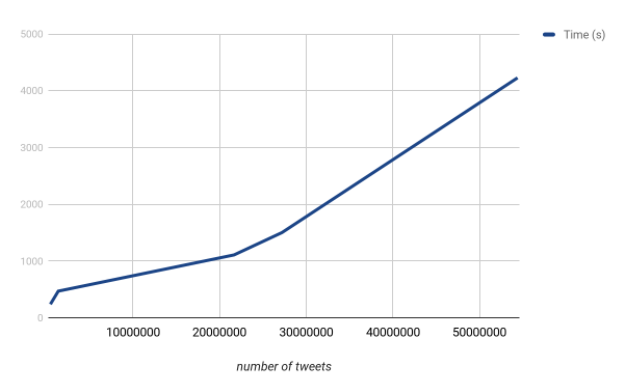
\includegraphics[width=\textwidth]{Figures/wordcountplot}
\decoRule
\caption[Wordcount time plot]{Plot on wordcount time for dataset size}
\label{fig:wordcountplot}
\end{figure}

To solve this tradeoff, we could move the index to primary key, adding an incrementing partition key to balance distribution between nodes similarly as random key. This is inspired to the column family distribution proposed in the work by Ahmet Arif, but using structured rows for each tweet instead of multiple JSON objects on each column. However due to the work being more focused on the container infrastructure part and concept development, this could not be performed during this thesis work.

On the other side, the current EPIC infrastructure is mainly oriented to collect tweets. Analysis are performed in dedicated machines that have a high number of cores and high RAM memory. In EPIC, mainly most of this analysis are performed in EPIC Analytics. However we need to take into account that due to the structure of the current system, batch analytics are performed after data has been extracted from Cassandra and therefore we can’t fully compare both system in terms of time to obtain a result since tweet collection. The current EPIC infrastructure is prepared to answer queries extracting data and running batch analysis. 

\begin{table}
\centering
\begin{tabular}{l l}
\toprule
\textbf{Number of tweets} & \textbf{Time (s)} \\
\midrule
490199 & 238 \\
1400884 & 469 \\
21680851 & 1107 \\
27199614 & 1500 \\
54395957 & 4228 \\
\bottomrule\\
\end{tabular}

\caption{Number of tweets in dataset vs seconds took to perform word count}
\label{tab:numtweets}
\end{table}

To solve this tradeoff, we could move the index to primary key, adding an incrementing partition key to balance distribution between nodes similarly as random key. This is inspired to the column family distribution proposed in the work by Ahmet Arif\parencite{batchreal}, but using structured rows for each tweet instead of multiple JSON objects on each column. However due to the work being more focused on the container infrastructure part and concept development, this could not be performed during this thesis work.

On the other side, the current EPIC infrastructure is mainly oriented to collect tweets. Analysis are performed in dedicated machines that have a high number of cores and high RAM memory. In EPIC, mainly most of this analysis are performed in EPIC Analytics. However we need to take into account that due to the structure of the current system, batch analytics are performed after data has been extracted from Cassandra and therefore we can’t fully compare both system in terms of time to obtain a result since tweet collection. The current EPIC infrastructure is prepared to answer queries extracting data and running batch analysis. 


\section{Real time analytics}

Real-time analysis has been approached before in the Project EPIC\parencite{batchreal}. However the previously mentioned approaches have a limited number of queries that can be answered in real time. Adding new queries would mean having to refactor the code and deploy again. The data used would also start to be collected once it’s deployed. Even though this approach gives result in a really low time, it lacks flexibility when it comes to custom queries. If analysts want custom queries, they would have to download the datasets and run their own custom analysis. This approach can be difficult, we need to predict what are the queries that we will need to answer ahead of time and sometimes this can be close to impossible.

For the new system, we took a more flexible approach. In order to increase flexibility, we sacrifice response time. Queries can be run on Spark while data is being collected, which makes their results near-real-time. We have a delay between when we start the query and when it ends, meaning that new data may have arrived during the query execution may have not been taken into account. 

This approach may seem as a lost in performance. However if analysts need custom analysis, this approach grants them a faster option. In addition, we allow for the analyst to run the query in an already existing system, which allows for the analysts to avoid having to configure their own system. Finally, thanks to the system decoupled architecture, it is possible in the future to add some real-time analysis by adding new consumers in the raw\_tweets queue that perform the mentioned static analysis, allowing for the existing feature in the current system to be re-deployed back in the new system.

\section{Software development and maintenance}

One of our goals was to develop a system that was easier to maintain. That was one of the reasons to adapt microservices was to avoid having components get outdated by making it easier for developers to onboard on the code and maintain it. In addition we also want to compare how easy would be to replace a component and code it from the ground up.

\subsection{Current infrastructure}

Currently the code is divided in 2 big monoliths. This can be a disadvantage on terms that developers must dig into the code of at least one of them in order to perform maintenance. This can be an small overhead as both of the projects are quite big. 

EPIC Analyze has 5086 lines of code. On boarding this part can be difficult. Specially since it uses a pretty closed framework as Ruby on Rails is. This can be a difficulty in terms of having to write new code, anyone who wants to write something need to learn the usage of Ruby on Rails. This framework is big and has a quite fast learning curve. However, it can be difficult as it implements practices that sometimes are not obvious for a developer coming from other frameworks. In addition to the code, we have a slow deployment process. In order to update the deployed version of EPIC Analyze, we need to restart the server manually. This makes it difficult to deploy, which in result turns into a really slow development process. Development for Analyze happens on a git repository, this makes collaboration easier between different developers.

EPIC Collect is difficult to analyze as it’s not on a git repository. Written in Java it’s built thinking on efficiency first.  This can be a bit of a difficulty in terms of collaborating and maintaining the code. In addition deploying new versions involves a lot of effort as it doesn’t only involve deploying the code, but also maintain the Tomcat server. We also need to take into account all the processes that are keeping EPIC Collect alive. Due to the fact that this scripts are embedded onto the development of EPIC Collect, we need to redeploy them manually.

\subsection{Proposed infrastructure}

The proposed infrastructure is divided into multiple different pieces. On one side we have the components code, divided between Python and Go code. On the other side we have the declaratives documents on YAML that specify how to deploy the infrastructure into Kubernetes.

\begin{itemize}
	\item \textit{Twitter tracker (Go)}: 108 lines 
	\item \textit{Kubernetes controller (Python)}: 145 lines
	\item \textit{Event manager UI (Python/Django)}: 2090 lines
	\item \textit{Tweet normalizer (Python)}: 209 lines
\end{itemize}

Code is more equilibrated distributed between different parts. The good thing is that we are not tied into an specific and unique framework. Making code small makes it easier for other developers to understand the purpose of each component. In addition thanks to separating responsibilities into microservices we can make collaboration easier by letting different developers work on different parts without crossing each other.

Something that also helps is that we can use different technologies in each component. This means that we can focus on building on the best available option for what we need to do. It also allows for a better pivoting of a component into a language that the maintainer prefers. If it can be containerized then it doesn’t matter what language or technology stack we use. It will be easily deployed into Kubernetes.

Finally we have the YAML files that store how the Kubernetes system looks like. All the system is declared in 3345 lines. There are many tools being released that will help make this code smaller. However right now the best option is to manually write and review each component in Kubernetes YAML files.


